We now present the scalability results relative to training InceptionV3~\cite{inception3}, a deep neural network by Google, on GPU-enabled nodes in Piz Daint and in Amazon EC2.\\
To do so, we use Google's script~\cite{cnn_benchmarks}, which provides optimized implementations for multiple networks.
The dataset used for training is ImageNet~\cite{imagenet}, one of the most common datasets used for classification in Computer Vision.\\

The code for this section can be found in the \texttt{google-benchmarks} folder of our repository.

\subsection{Methodology}
Google's script allows to set different parameters, such as the batch size, the number of warmup steps, the number of steps to be averaged, whether to use NVIDIA NCCL all-reduce primitives and the data layout format (NCHW or NHWC).\\

The main output of this script is the average number of images per second that have been trained in the system.
In order to find a good ratio between the number of Workers and the number of Parameter Servers, we try, for each configuration of number of Workers and number of nodes, several values for the number of PSs ranging from $1$ to the number of Workers.
For each configuration, we then report the results achieving the largest number of images trained per second.
In order to produce results that are as repeatable as possible, each test was run 5 times and then the times were averaged together, analogously to what Google did. 
GPUs are run in their default state on all the platforms.\\
For each test, 10 warmup steps are done and then the next 100 steps are averaged.\\

We ran our benchmarks using both real and synthetic data~\footnote{By synthetic data we mean fake data that has almost the same properties as the real one.}, so that we can evaluate both the compute and the input pipelines.

\subsection{Systems}
We run benchmarks on Piz Daint, as well as on \textit{p2.xlarge} and \textit{p2.8xlarge} Amazon EC2 instances.
Whenever possible, we compare our results with the ones published by Google~\cite{google_benchmarks}, obtained with \textit{NVIDIA DGX-1} and Amazon \textit{p2.8xlarge} systems.\\
Piz Daint and NVIDIA DGX-1 both have NVIDIA Tesla P100 GPUs, even though the former only has one GPU per node, while the latter has 8 GPUs per node.
Amazon \textit{p2.xlarge} and \textit{p2.8xlarge} EC2 instances, instead, are equipped with NVIDIA Tesla K80 GPUs. 
\textit{p2.xlarge} instances have one GPU per node, while \textit{p2.8xlarge} instances have eight GPUs per node (four K80).

\subsection{Results}
For all of the reported results, the following settings are used: 
\begin{itemize}
	\item \textbf{Model:} InceptionV3
	\item \textbf{Batch size per GPU:} 64
    \item \textbf{Data Format:} NCHW
    \item \textbf{Local Parameter Device:} CPU
	\item \textbf{Optimizer:} sgd
    \item \textbf{Piz Daint OS:} Suse 12/CLE 6.0.UP02
    \item \textbf{AWS OS:} Ubuntu 16.04 LTS
    \item \textbf{CUDA/cuDNN:} 8.0/5.1
    \item \textbf{TensorFlow:} 1.1.0
    \item \textbf{Piz Daint Parallel File System:} Lustre
    \item \textbf{AWS Disk:} Local SSD
    \item \textbf{DataSet:} ImageNet
	\item \textbf{Test Date:} August 2017
\end{itemize}
Moreover, nodes running Workers also run Parameter Servers as this leads to higher performance.

\subsubsection{Training with NVIDIA Tesla P100}
Google provides results only for a single NVIDIA DGX-1, hence allowing comparisons up to 8 GPUs.
Results are shown in Figure \ref{fig:dgx-daint} for synthetic data (no I/O).
\begin{figure}[t]
  \centering
  \includegraphics[width=\textwidth,trim={4cm 1.2cm 4.5cm 1.7cm},clip]{google-daint-synthetic.pdf}
  \vspace{-0.85cm}
  \caption{Training with NVIDIA Tesla P100 on synthetic data up to 8 GPUs.} 
  \label{fig:dgx-daint}
\end{figure}
Here, we can see that the peak performance of Piz Daint is close to the one achieved by an NVIDIA DGX-1, even though multiple nodes are used in Piz Daint.
Specifically, with eight GPUs, while Google reports a speedup efficiency of $99.56\%$, we report a speedup efficiency of $92.07\%$ on Piz Daint.

\vspace{-0.3cm}
\subsubsection{Training with NVIDIA Tesla K80}
\vspace{-0.2cm}
Figure \ref{fig:aws-google-cscs} shows how Amazon EC2 \textit{p2.xlarge} and \textit{p2.8xlarge} compute instances scale out up to 8 GPUs.
\begin{figure}[H]
  \centering
  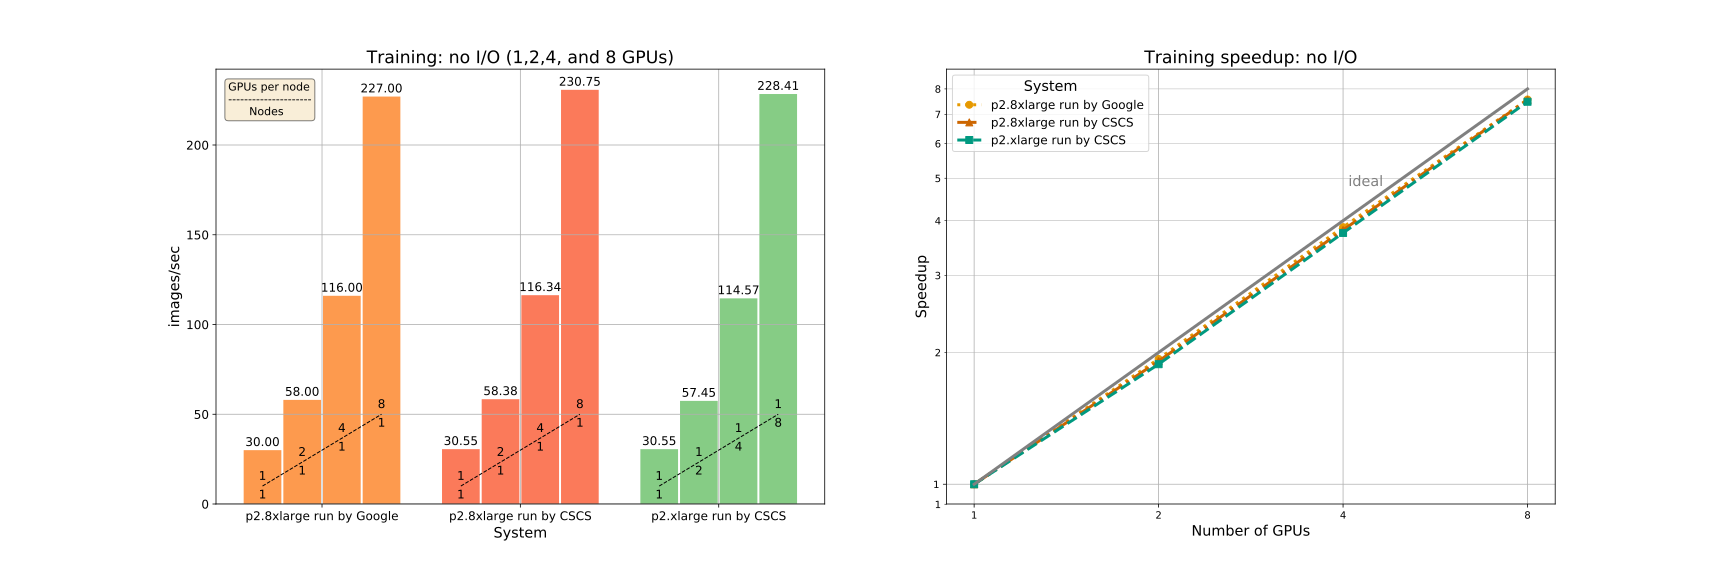
\includegraphics[width=\textwidth,trim={4cm 1.2cm 4.5cm 1.7cm},clip]{google-our-aws-synthetic.pdf}
  \vspace{-0.85cm}
  \caption{Training with NVIDIA Tesla K80 on synthetic data up to 8 GPUs.} 
  \label{fig:aws-google-cscs}
\end{figure}
\vspace{-0.2cm}
Google provides results that achieve a scalability efficiency of $94.58\%$ with 8 GPUs on a \textit{p2.8xlarge}, and, similarly, our measurements show an efficiency of $94.44\%$ on the same machine.\\
We also ran tests on \textit{p2.xlarge} instances, showing that comparable performance ($93.45\%$ scalability efficiency) can be obtained with eight nodes (eight GPUs).\\
Hence, we can infer that the application is compute bounded when up to eight GPUs are used because we achieve the same performance with eight nodes as with a single node having eight GPUs regardless of the underlying network (Piz Daint or AWS).\\

Figure \ref{fig:dist-aws-google-cscs}, instead, shows how the number of images trained per second in these systems scales when up to 64 GPUs are used.
\begin{figure}[t]
  \centering
  \includegraphics[width=\textwidth,trim={4cm 1.2cm 4.5cm 1.7cm},clip]{google-our-dist-aws-synthetic.pdf}
  \vspace{-0.85cm}
  \caption{Training with NVIDIA Tesla K80 on synthetic data up to 64 GPUs.} 
  \label{fig:dist-aws-google-cscs}
\end{figure}
% \vspace{-0.5cm}
It is interesting to note that up to 16 GPUs, \textit{p2.xlarge} and \textit{p2.8xlarge} systems have close performance: We report $88.31\%$ for the former and $91.77\%$ for the latter.\\
Moreover, even though 32 nodes are required for a \textit{p2.xlarge} system to use 32 GPUs, it still achieves a scalability efficiency greater than $80\%$.
Specifically, we report $88.35\%$ efficiency for a four-node \textit{p2.8xlarge} system and $84.45\%$ efficiency for a thirty-two-node \textit{p2.xlarge} system.\\
However, once a cluster of sixty-four \textit{p2.xlarge} nodes is employed, the scalability efficiency stops at $50.96\%$, while a cluster of eight \textit{p2.8xlarge} still exhibits $88.55\%$ efficiency from our measurements and $92.86\%$ from Google's ones.
This is probably due to the fact that the network capacity is not sufficient anymore for the amount of traffic generated by all the nodes in the \textit{p2.xlarge} cluster.

\subsubsection{Distributed training on Piz Daint}
Figure \ref{fig:daint} shows how the average number of images trained per second varies as the number of nodes (GPUs) increases both when using fake data and when reading data from the Parallel File System on Piz Daint.
Each of these values represents the peak performance achieved with the corresponding number of GPUs, obtained by setting the parameters listed in Table \ref{tab:peak-perf-daint}.
Here, we can see that Piz Daint's scalability efficiency drastically drops when 128 nodes are used.
We think this is due to having reached the inter-node network capacity because of the largely increased amount of data sent between Workers and Parameter Servers.
\begin{figure}[H]
  \centering
  \includegraphics[width=\textwidth,trim={4cm 1.2cm 4.5cm 1.7cm},clip]{daint-synthetic-real.pdf}
  \vspace{-0.85cm}
  \caption{Training on Piz Daint with synthetic and real data up to 128 GPUs.} 
  \label{fig:daint}
\end{figure}
% \vspace{-0.5cm}
\begin{table}[H]
 \centering
 \begin{tabular}{||l | l | l | l | r||} 
 \hline
 \textbf{Num PSs} & \textbf{Num GPUs} & \textbf{Variable Update} & \textbf{Real Data} & \textbf{Img/s}\\ [0.5ex] 
 \hline\hline
 1 & 1 & parameter\_server & FALSE & 138.23\\\hline
 1 & 1 & parameter\_server & TRUE & 137.03\\\hline
 1 & 2 & parameter\_server & FALSE & 264.57\\\hline
 1 & 2 & distributed\_replicated & TRUE & 260.84\\\hline
 3 & 4 & distributed\_replicated & FALSE & 523.38\\\hline
 3 & 4 & distributed\_replicated & TRUE & 516.71\\\hline
 2 & 8 & parameter\_server & FALSE & 1018.18\\\hline
 2 & 8 & parameter\_server & TRUE & 911.84\\\hline
 4 & 16 & parameter\_server & FALSE & 2001.00\\\hline
 4 & 16 & parameter\_server & TRUE & 1772.34\\\hline
 12 & 32 & parameter\_server & FALSE & 3840.35\\\hline
 12 & 32 & parameter\_server & TRUE & 3425.55\\\hline
 40 & 64 & parameter\_server & FALSE & 7118.31\\\hline
 40 & 64 & parameter\_server & TRUE & 6348.74\\\hline
 116 & 128 & parameter\_server & FALSE & 9219.70\\\hline
 116 & 128 & parameter\_server & TRUE & 9055.64\\\hline
\end{tabular}
\caption{Parameters achieving peak performance on Piz Daint.}
\label{tab:peak-perf-daint}
\end{table}

\subsubsection{Distributed training on Amazon p2.xlarge}
Figure \ref{fig:p2} displays the trend of average number of images trained per second as the number of nodes (GPUs) increases both when using fake data and when reading data from the local SSD at each node in a cluster of \textit{p2.xlarge} machines.
The parameters resulting in the peak performance for each different number of GPUs are listed in Table \ref{tab:peak-perf-p2}.
In this plot, we can see that \textit{p2.xlarge}'s scalability efficiency diminishes only when 64 nodes are benchmarked.
This system has single-GPU nodes like Piz Daint but it stops scaling out efficiently for a smaller number of nodes.
The main difference amongst them is their inter-node network (Piz Daint's being faster), providing additional support to our belief of inter-node network bottleneck for Piz Daint and \textit{p2.xlarge} systems.
\begin{figure}[H]
  \centering
  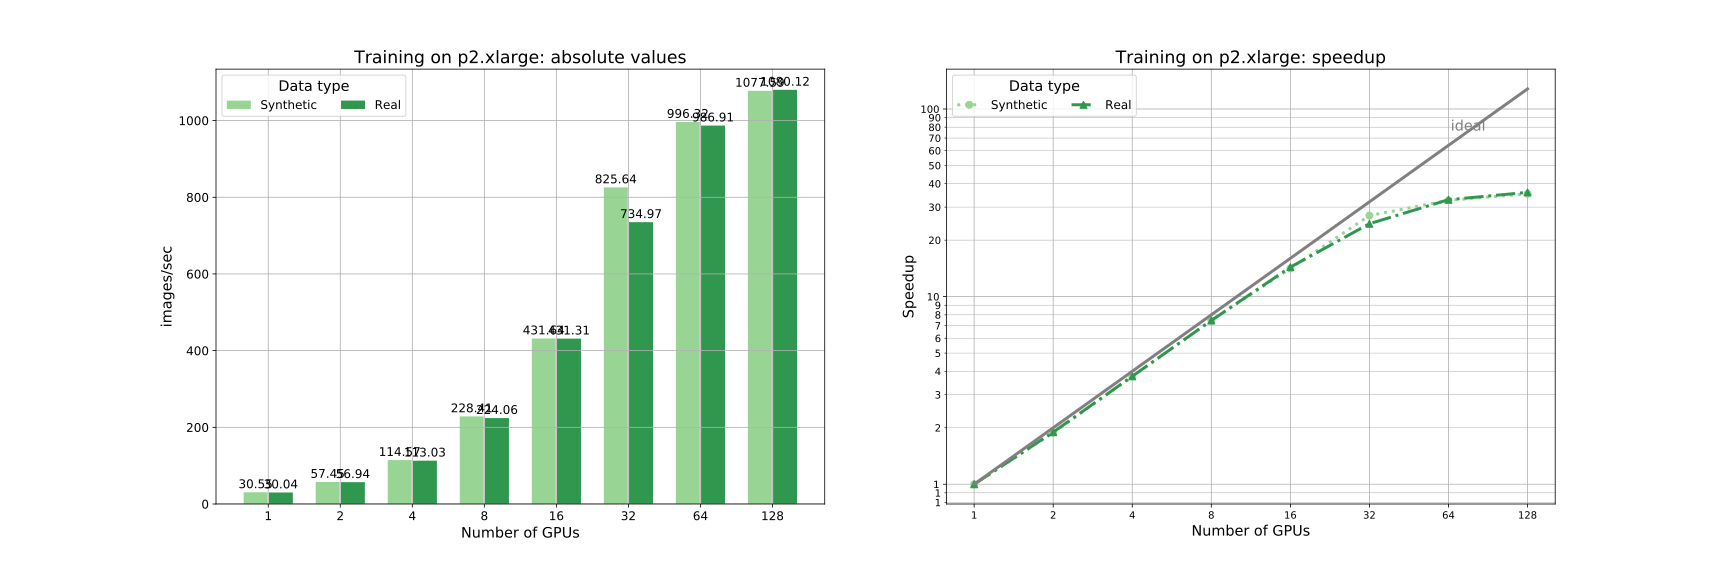
\includegraphics[width=\textwidth,trim={4cm 1.2cm 4.5cm 1.7cm},clip]{p2-synthetic-real.pdf}
  \vspace{-0.85cm}
  \caption{Training on \textit{p2.xlarge} with synthetic and real data up to 128 GPUs.}
  \label{fig:p2}
\end{figure}
% \vspace{-0.5cm}
\begin{table}[H]
 \centering
 \begin{tabular}{||l | l | l | l | r||} 
 \hline
\textbf{Num PSs} & \textbf{Num GPUs} & \textbf{Variable Update} & \textbf{Real Data} & \textbf{Img/s}\\ [0.5ex] 
\hline\hline
 1 & 1 & parameter\_server & FALSE & 30.55\\\hline
 1 & 1 & parameter\_server & TRUE & 30.04\\\hline
 2 & 2 & distributed\_replicated & FALSE & 57.45\\\hline
 2 & 2 & distributed\_replicated & TRUE & 56.93\\\hline
 4 & 4 & distributed\_replicated & FALSE & 114.57\\\hline
 4 & 4 & distributed\_replicated & TRUE & 113.03\\\hline
 8 & 8 & distributed\_replicated & FALSE & 228.41\\\hline
 8 & 8 & distributed\_replicated & TRUE & 224.06\\\hline
 12 & 16 & distributed\_replicated & FALSE & 431.64\\\hline
 12 & 16 & distributed\_replicated & TRUE & 431.31\\\hline
 32 & 32 & parameter\_server & FALSE & 825.64\\\hline
 32 & 32 & parameter\_server & TRUE & 734.97\\\hline
 64 & 64 & parameter\_server & FALSE & 996.32\\\hline
 64 & 64 & parameter\_server & TRUE & 986.91\\\hline
 128 & 128 & parameter\_server & FALSE & 1077.59\\\hline
 128 & 128 & parameter\_server & TRUE & 1080.12\\\hline
\end{tabular}
\caption{Parameters achieving peak performance on \textit{p2.xlarge} systems.}
\label{tab:peak-perf-p2}
\end{table}

\subsubsection{Distributed training on Amazon p2.8xlarge}
\vspace{-0.2cm}
Figure \ref{fig:p28} presents the average number of images trained per second as a function of the number of GPUs both when using fake data and when reading data from local the SSD at each node in a \textit{p2.8xlarge} cluster.
The parameters giving the highest performance for the different numbers of GPUs are enlisted in Table \ref{tab:peak-perf-p28}.
This plot does not show any evident reduction in scalability as the number of GPUs is increased.
In such system, Workers aggregate their updates before sending them to the PSs. 
Hence, the traffic generated when 128 GPUs are used here is comparable to the one generated by a system of sixteen single-GPU nodes.
\vspace{-0.2cm}
\begin{figure}[H]
  \centering
  \includegraphics[width=\textwidth,trim={4cm 1.2cm 4.5cm 1.7cm},clip]{p28-synthetic-real.pdf}
  \vspace{-0.85cm}
  \caption{Training on \textit{p2.8xlarge} with synthetic and real data up to 128 GPUs.}
  \label{fig:p28}
\end{figure}
\vspace{-0.55cm}
\begin{table}[H]
 \centering
 \begin{tabular}{||l | l | l | l | r||} 
 \hline
 \textbf{Num PSs} & \textbf{Num GPUs} & \textbf{Variable Update} & \textbf{Real Data} & \textbf{Img/s}\\ [0.5ex]  
 \hline\hline
 1 & 1 & parameter\_server & FALSE & 30.55\\\hline
 1 & 1 & parameter\_server & TRUE & 30.04\\\hline
 1 & 2 & distributed\_replicated & FALSE & 58.38\\\hline
 1 & 2 & distributed\_replicated & TRUE & 58.23\\\hline
 1 & 4 & distributed\_replicated & FALSE & 116.34\\\hline
 1 & 4 & distributed\_replicated & TRUE & 115.56\\\hline
 1 & 8 & distributed\_replicated & FALSE & 230.75\\\hline
 1 & 8 & distributed\_replicated & TRUE & 190.02\\\hline
 1 & 16 & distributed\_replicated & FALSE & 448.57\\\hline
 1 & 16 & distributed\_replicated & TRUE & 387.67\\\hline
 3 & 32 & distributed\_replicated & FALSE & 863.72\\\hline
 3 & 32 & distributed\_replicated & TRUE & 717.49\\\hline
 8 & 64 & distributed\_replicated & FALSE & 1731.31\\\hline
 8 & 64 & distributed\_replicated & TRUE & 1430.28\\\hline
 16 & 128 & distributed\_replicated & FALSE & 3333.20\\\hline
 16 & 128 & distributed\_replicated & TRUE & 2832.83\\\hline
\end{tabular}
\caption{Parameters achieving peak performance on \textit{p2.8xlarge} systems.}
\label{tab:peak-perf-p28}
\end{table}

\subsubsection{I/O overhead}
Finally, Figure \ref{fig:io} plots the relative overhead (in percentage) due to I/O access.
That is, for each setting, we obtain the relative I/O in percentage as:
$$I/O~overhead~_{System}^{N\_GPUs} = \dfrac{Img/s\_Synthetic_{System}^{N\_GPUs} - Img/s\_Real_{System}^{N\_GPUs}}{Img/s\_Synthetic_{System}^{N\_GPUs}} \times 100.$$

The first thing we observe from this plot is that when 8 GPUs per node are used in a \textit{p2.8xlarge} cluster, where each node loads data from a local SSD, a constant I/O overhead of around $17\%$ is present (due to PCIe traffic).\\

Looking at \textit{p2.xlarge} clusters, instead, we see that I/O access does not add any overhead, apart when thirty-two nodes are used.
However, this still comes at the expenses of replicating the data at each node.\\

Focusing on Piz Daint at last, we see that around $11\%$ of I/O overhead is present when eight to sixty-four nodes are used.\\
On the other hand, this is not shown when less nodes are employed.
The reason might be due to caching mechanisms in the system.\\
The I/O overhead drops down once more for one hundred and twenty-eight nodes.
In this case, the reason of this reduction may be found in the predominance of the inter-node network bottleneck, which makes the impact of I/O access negligible.\\

TensorFlow communication patterns should be profiled to verify all our intuitions.

\begin{figure}[t]
  \centering
  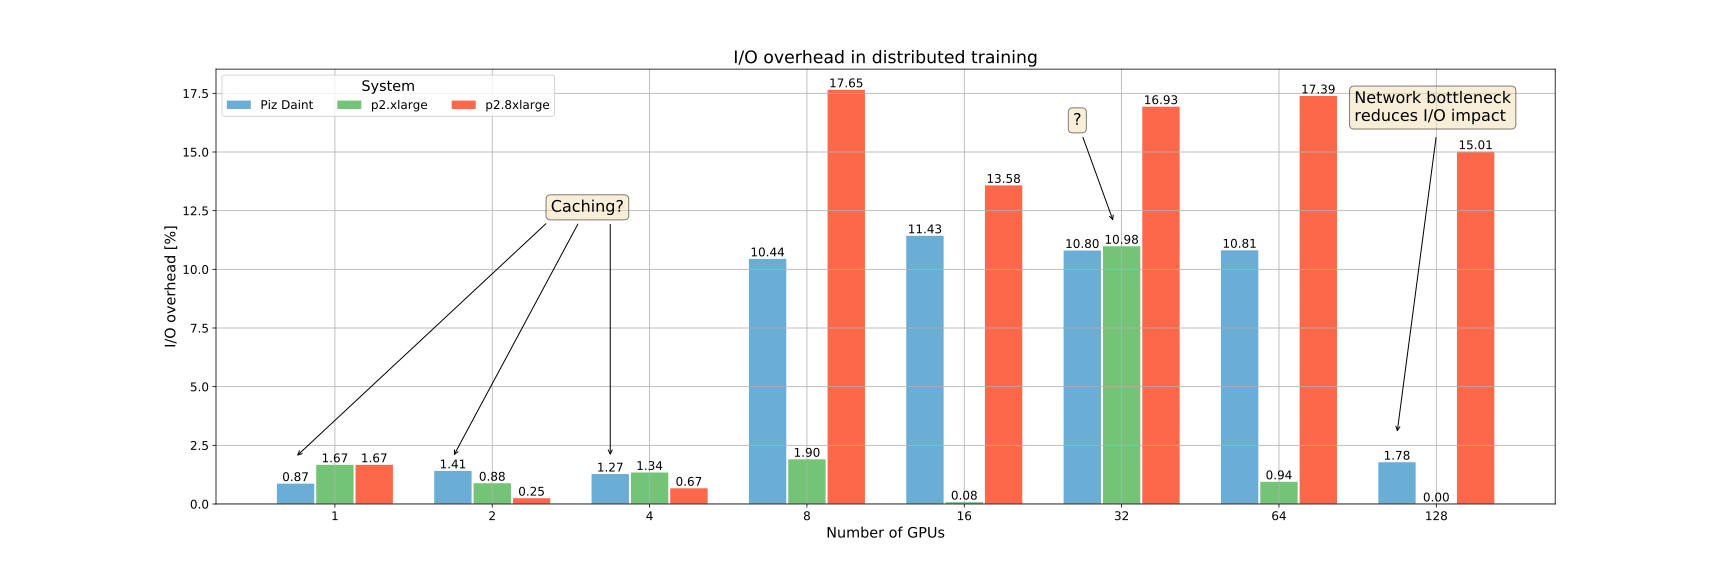
\includegraphics[width=\textwidth,trim={4cm 1.2cm 4.5cm 1.7cm},clip]{io-synthetic-real.pdf}
  \vspace{-0.85cm}
  \caption{I/O overhead in distributed training in terms of number of GPUs for all the systems under study.} 
  \label{fig:io}
\end{figure}
\vspace{-0.5cm}